\section{Organisation du contenu du manuscrit}\label{sec:intro:outline}

\begin{figure}[h!]
  \centering
  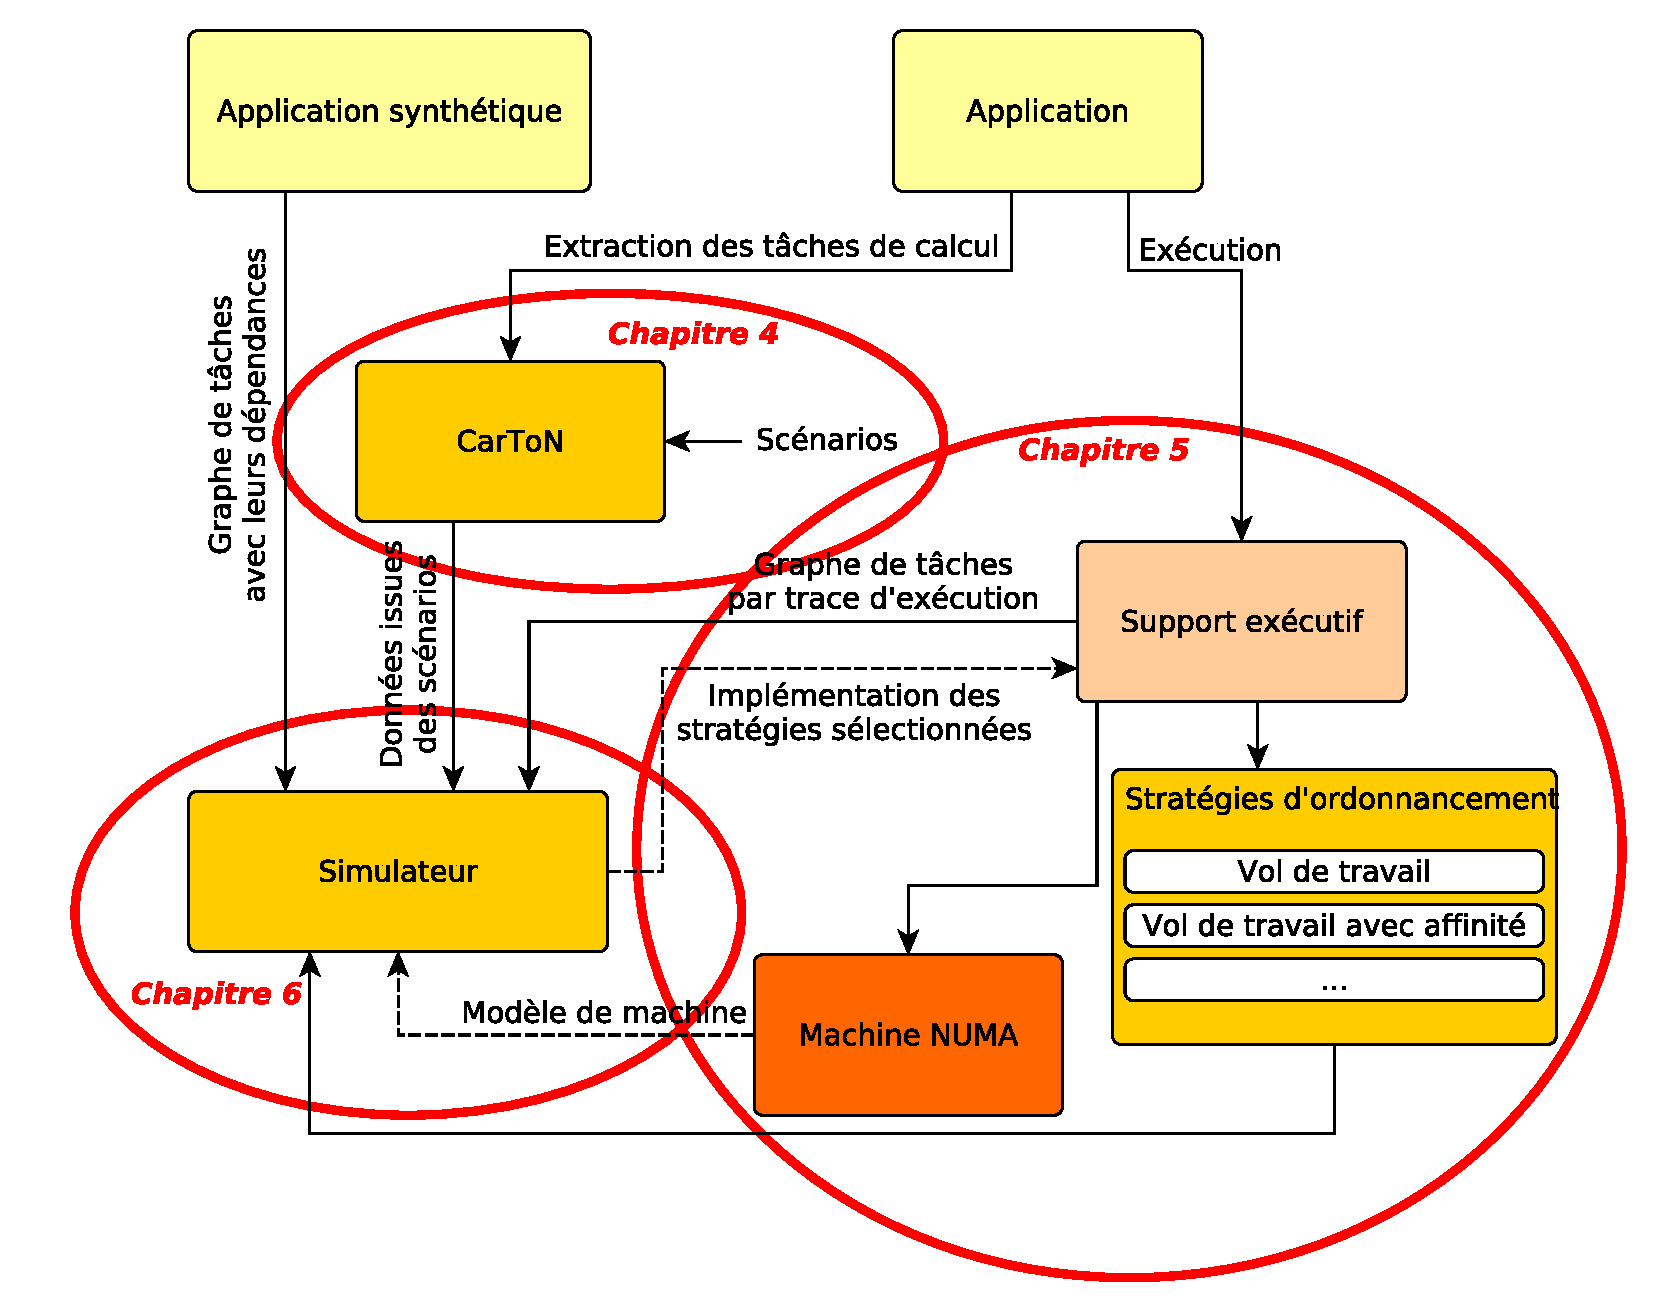
\includegraphics[width=\textwidth]{big_picture_annotated}
  \caption{Vision schématique des différentes contributions de la thèse}\label{fig:intro:big_picture_annotated}
\end{figure}

Le manuscrit est découpé en deux grandes parties.
La première partie traite des problématiques abordées par cette thèse, ainsi que des approches existantes sur les points techniques abordés.
Dans cette partie, le chapitre~\ref{chap:contexte} introduit les éléments de base nécessaires au déroulement de cette thèse : les architectures à mémoire partagée, les moyens existants de les programmer, et une description détaillée de certains outils et concepts techniques fondamentaux.
Le chapitre~\ref{chap:rw} revient sur l'état de l'art des techniques utilisées ou étendues par nos travaux.

La seconde partie regroupe nos travaux sur l'étude des machines NUMA, et l'amélioration de leur utilisation à travers OpenMP.
La figure~\ref{fig:intro:big_picture_annotated} illustre les différentes contributions de cette thèse ainsi que leurs interactions.
Le chapitre~\ref{chap:contrib:characterization} introduit \outil, un outil que nous avons créé pour étudier en détails le comportement des applications et de l'architecture sous jacente~; nous décrivons également l'orientation des travaux à la suite de nos observations.
Les extensions du langage et du support exécutif sont motivées, décrites et évaluées dans le chapitre~\ref{chap:contrib:openmp}.
Le chapitre~\ref{chap:simulation} décrit un prototype de simulateur que nous avons écrit afin d'analyser et d'envisager de nouvelles stratégies d'ordonnancement, à partir notamment des données issues des expériences effectuées avec \outil.

Enfin le chapitre~\ref{chap:conclusion} se concentre sur les perspectives et revient sur l'évolution du matériel et du logiciel pendant la thèse, et discute des pistes de recherche envisageables pour pousser plus loin nos idées, avant de conclure notre travail et ce manuscrit.
